\documentclass[14pt,a4paper]{scrartcl}
\usepackage[utf8]{inputenc}
\usepackage[english,russian, ukrainian]{babel}
\usepackage{misccorr, color, ragged2e, amsfonts, amsthm, graphicx, systeme, amsmath, mdframed, lipsum, setspace, mathtools, esint, color, listings}

\renewcommand\qedsymbol{$\blacksquare$}
\renewcommand*{\proofname}{\text{Доведення}}

\theoremstyle{definition}
\newtheorem*{defo}{Означення}
\newtheorem*{teo}{Теорема}
\newtheorem*{example}{Приклад}
\theoremstyle{remark}
\newtheorem*{remark}{Зауваження}
\theoremstyle{definition}
\newtheorem*{consequence}{Наслідок}
\theoremstyle{definition}
\newtheorem{statement}{Утверждение}[section]
\newmdtheoremenv{boxteo}{Теорема}[section]
\newtheorem*{look}{Позначення}

\setlength\parindent{0pt}

\DeclareMathOperator*\lowlim{\underline{lim}}
\DeclareMathOperator*\uplim{\overline{lim}}

\newcommand\independent{\protect\mathpalette{\protect\independenT}{\perp}}

\def\independenT#1#2{\mathrel{\rlap{$#1#2$}\mkern2mu{#1#2}}}

% Default fixed font does not support bold face
\DeclareFixedFont{\ttb}{T1}{txtt}{bx}{n}{12} % for bold
\DeclareFixedFont{\ttm}{T1}{txtt}{m}{n}{12}  % for normal

\definecolor{deepblue}{rgb}{0,0,0.5}
\definecolor{deepred}{rgb}{0.6,0,0}
\definecolor{deepgreen}{rgb}{0,0.5,0}

\doublespacing

\begin{document}

\def\be{\begin{equation}}
\def\ee{\end{equation}}

\def\bd{\begin{defo}}
\def\ed{\end{defo}}

\def\bbt{\begin{boxteo}}
\def\ebt{\end{boxteo}}

\def\i{\infty}
\def\d{\partial}

\def\vx{\overline{x}}
\def\vphi{\overline{\varphi}}
\def\vf{\overline{f}}

\begin{titlepage}
\begin{center}

\vspace*{0.1cm}
\vfill

\begin{spacing}{3}
  {\huge \textbf{ТЕОРІЯ СТІЙКОСТІ \\ ТА ВАРІАЦІЙНЕ ЧИСЛЕННЯ}}\\
\end{spacing}
\vspace{5cm}
За лекціями Горбань Н.\\
\vspace{1cm}
Редактори: Терещенко Д.\\ \hspace{3.7cm} Людомирський Ю.

\vfill

2021

\end{center}
\end{titlepage}


\tableofcontents
\newpage

\section{Лекція 1}
\subsection{Нормальні системи диференційних рівнянь}


\be
\left\lbrace
\begin{gathered}
    x'_1 (t) = f_1(t, x_1 (t), ... , x_n(t)) \\
    x'_2 (t) = f_2(t, x_1 (t), ... , x_n(t)) \\
    \vdots \\
    x'_n (t) = f_n(t, x_1 (t), ... , x_n(t)) \\
\end{gathered}\right.
\ee

 Системою диф. рівнянь n-го порядку в нормальній формі називається система вигляду (1), де $ f_i : D \to \mathbb{R}, \quad D \subset \mathbb{R}^{n+1 }, \quad i = \overline{1, n}$.
\look
\[
      \overline{x}(t) = \left[\begin{array}{l}
      x_1(t)    \\
      \dots     \\
      x_n(t)
      \end{array}\right] \text{-- невідома вектор-функція}, \quad
      \overline{f}(t, \overline{x}(t)) = \left[\begin{array}{l}
      f_1     \\
      \dots  \\
      f_n
      \end{array}\right] \text{, що}
\]
$D \rightarrow \mathbb{R}, \quad D \subset \mathbb{R}^{n+1}$, тоді $(1): \overline{x}'(t) = \overline{f}(t, \overline{x}(t))$.


\def\rect{\textbf{П}}
\bd
\textbf{Розв'язком системи} (1) на $(\alpha , \beta)$ називається така вектор-функція $\overline{x} (t) \in C^1(\alpha , \beta)$, що:
\begin{enumerate}
  \item $(t, x_1(t), \dots, x_n(t)) \in D \quad \forall t \in (\alpha, \beta)$;
  \item $\overline{x}(t)$  перетворює $(1)$ на тотожність на інтервалі $(\alpha, \beta)$.
\end{enumerate}

\textbf{Загальним розв'язком системи}  (1) називається n-параметрична сім'я розв'язків (1), що охоплює всі розв'язки системи.
\ed

Задача Коші. Для заданих $t_0, \overline{x}^{0} \in D$ знайти такий розв'язок (1), що $\overline{x} (t_0) = \overline{x}^{0}$.
Нехай $\Pi = \{(t, \overline{x}) \in \mathbb{R} \quad \big| \quad |t-t_0| \leq a, \quad ||\overline{x} - \overline{x}_0|| \leq b \}$.

\begin{boxteo}[Теорема Пеано]
Нехай $\vec{f} \in C(\Pi)$. Тоді розв'язок задачі Коші:
\begin{gather*}
  \begin{cases}
    \overline{x}' = \overline{f}(t, \overline{x}) \\
    \overline{x}(t_0) = \overline{x}_0
  \end{cases}
\end{gather*}
існує принаймні на проміжку $I_h = (t_0 - h, t_0 + h)$, де $h = \min\{{a, \dfrac{b}{M}}\}$, \\ $M = \max\limits_{(t, x) \in \Pi} {||\overline{f}(t, \overline{x})||}$.
\end{boxteo}

\begin{boxteo}[про продовження]
Нехай для системи (1) виконується, що $\overline{f} \in C(D), \quad D \subset \mathbb{R}^{n + 1}$ -- обмежена область. Тоді $\forall t : (t_0, \overline{x}_0) \in D$ існують такі $t^{-}, t^{+} : t^{-} < t_0 < t^{+}$, що розв'язок системи (1) з початкової умови $\overline{x}(t_0) = \overline{x}_0$ існує на інтервалі $(t^{-}, t^{+})$, причому $(t^{-}, \overline{x}(t^{-})) \text{ та } (t^{+}, \overline{x}(t^{+}))$ належать межі області $D$.
    \begin{center} 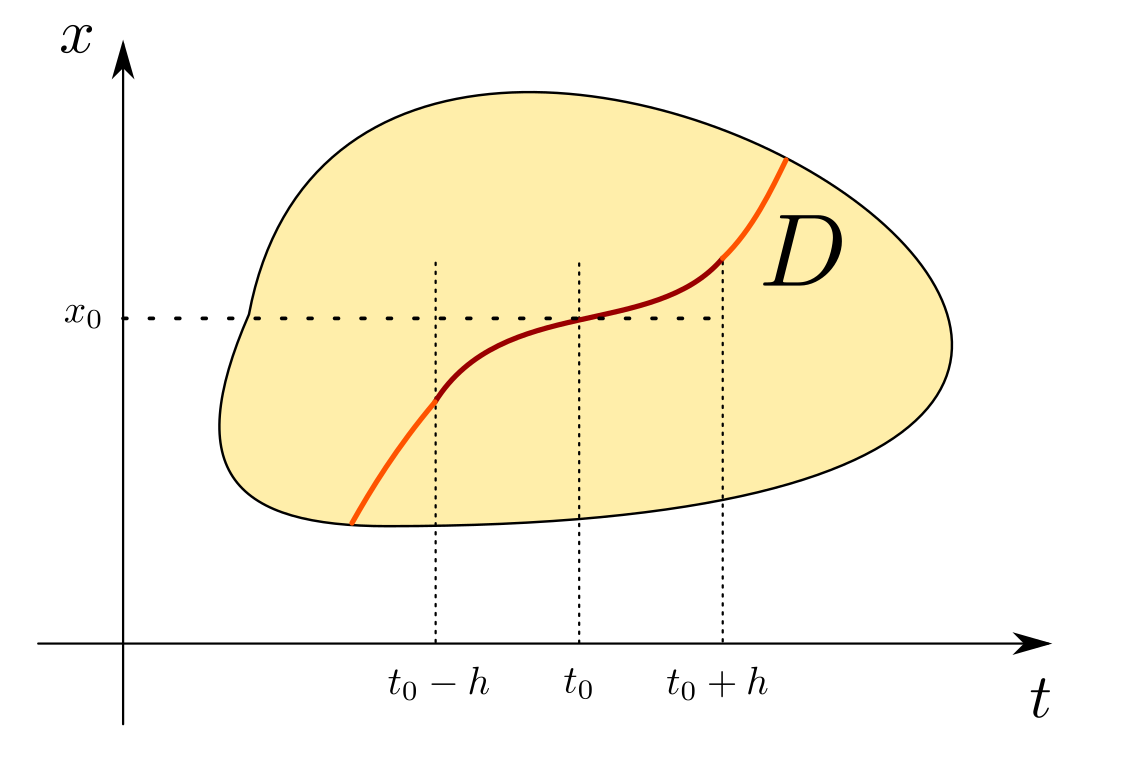
\includegraphics[scale=0.35]{assets/lect0.png} \end{center}
\end{boxteo}

\begin{boxteo}[Теорема Пікара]
  Нехай
  \begin{spacing}{1}
  \begin{enumerate}
    \item $\overline{f} \in C(\Pi)$;
    \item $\exists! L > 0 : \forall (t_1, \overline{x}_1), (t_2, \overline{x}_2) \in \Pi$ справедливо, що $|| f(t_1, \overline{x}_1) - f(t_2, \overline{x}_2)|| \leq \\ \leq L||\overline{x}_1 - \overline{x}_2||$ (умова Ліпшиця).
  \end{enumerate}
  \end{spacing}


  Тоді $\exists!$ розв'язок задачі Коші з початкової умови $\overline{x}(t_0) = \overline{x}_0(t)$, визначений принаймні на $I_h = (t_0 - h, t_0 + h), \quad h = \min\{{a, \dfrac{b}{M}}\}, \quad M = \max\limits_{\Pi}||f(t, \overline{x})||$.
\end{boxteo}

\subsection{Основні поняття теорії стійкості.}
Розглянем систему диференційних рівнянь $\overline{x}' = \overline{f}(t, \overline{x})$ (1), де $f : D \rightarrow \mathbb{R}^n$ та $D = [a, +\infty] \times G, \quad G \subset \mathbb{R}^n$. Нехай при цьому $\overline{f}$ задавольняє умовам існування та єдиності розв'язку задачі Коші в будь-якій точці $(t_0, \overline{x}_0) \in D$

\bd
Розв'язок $\overline{x} = \overline{\varphi}(t)$ системи (1) називається \textbf{стійким} за Ляпуновим, якщо

\begin{enumerate}
  \item $\overline{x} = \overline{\varphi}(t) \quad \exists  \text{ на } [a, +\infty]$ (відсутніть вертикальних асимптот)
  \item $\forall \varepsilon > 0 \quad \forall t_0 \geq a \quad \exists \delta > 0 : \forall $ розв'язку $\overline{x}(t)$ системи (1) такого, що $||\overline{x}(t_0) - \overline{\varphi}(t_0)|| < \delta$ виконується наступне, що $\overline{x}(t)$ існує на $[t_0, +\infty]$ та $||\overline{x}(t) - \overline{\varphi}(t)|| < \varepsilon \quad \forall t \geq t_0$.
\end{enumerate}
\ed

\begin{center} 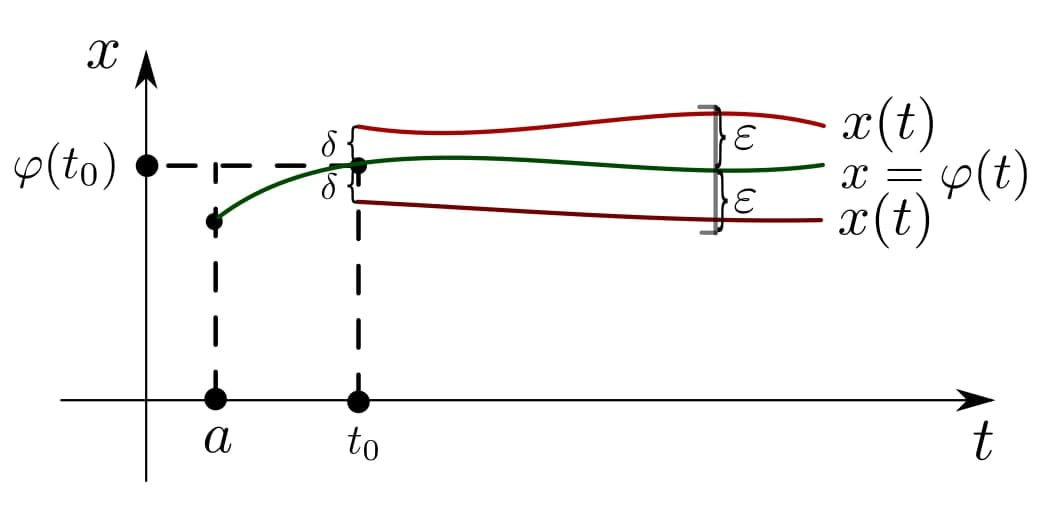
\includegraphics[scale=0.35]{assets/lect1.jpg} \end{center}

\bd
Розв'язок $\overline{x} = \overline{\varphi}(t)$ системи (1) називається \textbf{асимптотично стійким} за Ляпуновим, якщо

\begin{enumerate}
  \item $\overline{x} = \overline{\varphi}(t)$ стійкий;
  \item $\forall t_0 \geq a \quad \exists \delta > 0: \forall$ розв'язку $\vec{x}(t)$ с-ми (1) такого, що $||\vec{x}(t_0) - \vec{\varphi}(t_0)|| < \delta$ справедливо, що $||\vec{x}(t_0) - \vec{\varphi}(t_0)|| \rightarrow 0 \text{ при } t \rightarrow + \infty$.
\end{enumerate}

\begin{center} 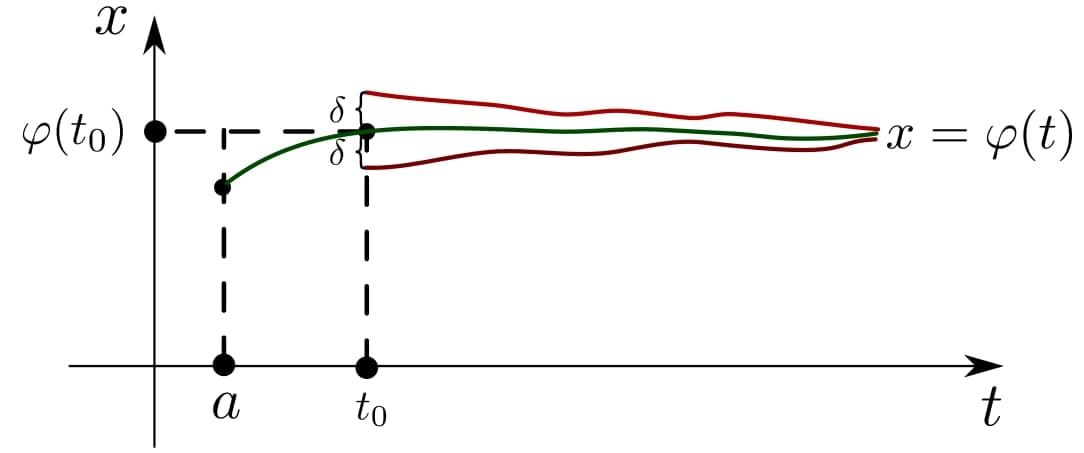
\includegraphics[scale=0.35]{assets/lect2.jpg} \end{center}

Роз'язок $\vec{\varphi}(t)$ називається \textbf{нестійким за Ляпуновим}, якщо він не є стійким, тобто:
\ed

\begin{enumerate}
  \item Або $\overline{x} = \overline{\varphi}(t) \quad \nexists$ на  $[a, +\infty]$ (вертикальні асимптоти);
  \item Або $\exists \varepsilon > 0 : \exists t_0 \geq a :  \forall \delta > 0$ існує розв'язок $\vec{x}(t)$ системи (1) такий, що $||\vec{x}(t_0) - \vec{\varphi}(t_0)|| < \delta$, але $||\vec{x}(t_0) - \vec{\varphi}(t_0)|| > \varepsilon$
\end{enumerate}

\begin{center} 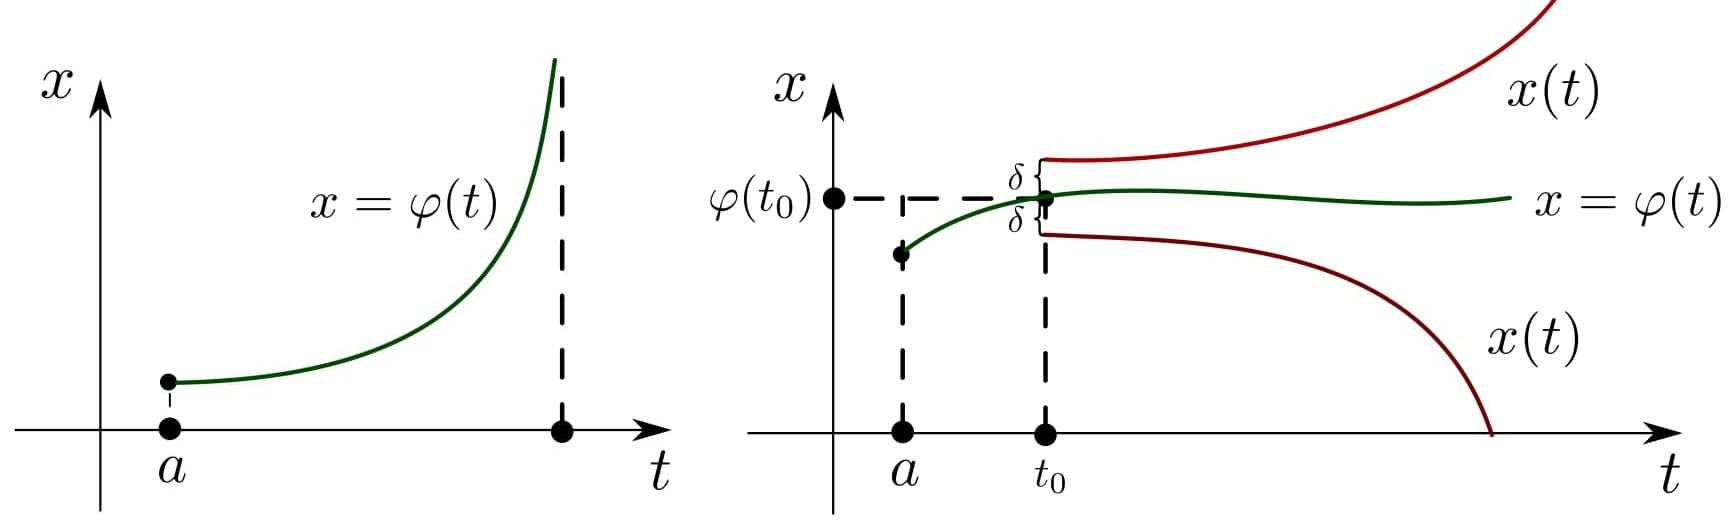
\includegraphics[scale=1.25]{assets/lect3+4.jpg} \end{center}

\subsection{Приклади дослідження на стійкість за означенням.}

\begin{example}
    Дослідити на стійкість розв'язок З.К.:
$$
\begin{cases}
    x = 1 \\
    x(0) = 0
\end{cases}
$$
1. Знайдемо розв'язок заданої З.К.: $x = 1 \Rightarrow x = t + C$ - заг. розв.\\
Підставимо: $ 0 = 0 + C \Longrightarrow C = 0 \Longrightarrow $ \fbox{ $ \varphi(t) = t $} - будемо досліджувати.
Зазначений розв'язок не має вертикальних асимптот та існує на всьому $\mathbb{R}$.
2. Знайдемо розв'язок довільної З.К. $x(t_0) = x_0$.
$$
x_0 = t_0 + C \Rightarrow C = x_0 - t_0 \Rightarrow x(t) = t + x_0 - t_0
$$
3. Нехай $  \left| x(t_0) - \varphi(t_0) \right|  =  \left| x_0 - t_0 \right| < \delta  $ ;\\
Тоді $ \left| x (t) - \varphi (t) \right|  = \left|  x_0 - t_0 \right| < \varepsilon = \delta $.\\
Таким чином, розв'язок є стійким, але не є асимптотично стійким.

\end{example}

\begin{example}
    Дослідити на стійкість розв'язок З.К.:
    $$
    \begin{cases}
        \dot{x} = 1 + t - x \\
        x(0) = 0
    \end{cases}
    $$
    1. Знайдемо розв'язок даної задачі Коші:
    $$
    \dot{x} = - x + 1 + t = \left| \text{ методом Бернуллі } \right| = t + Ae^{-t}
    $$
    Знайшли загальний розв'язок. Підставимо умову із з. К.: $ A = 0 \Rightarrow \fbox {$\varphi(t) = t$ }$\\
    2. Знайдемо розв'язок довільної З.К.:
    $$
    x(t_0) = x_0 \qquad x_0 = t_0 + Ae^{-t_0} \qquad A = (x_0 - t_0) e^{t_0}
    $$
    $$
    x(t) = t + (x_0 - t_0) e^{t_0 - t} - \text{ загальний розв'язок з. К.}
    $$

    3. Нехай $ \left|  x(t_0) - \varphi(t_0)  \right| = \left| x_0 - t_0 \right|  < \delta $. Розглядаємо: $ \forall t \geq t_0 :$
    $$
    \left| x(t) - \varphi(t) \right| = \left| t + (x_0 - t_0) \cdot e^{ t_0 - t} - t \right| =
     \left| x_0 - t_0 \right|< \delta  \to 0  \quad (t \to + \infty)
    $$
    Отримали, що знайдений розв'язок є асимптотично стійким.
\end{example}
Перейдемо знов до систем диф. рівнянь: $ \vx' = \vf (t, \vx)  \quad (1)$.\\
$\vx = \vphi (t)$ - розв'язок, який ми маємо дослідити на стійкість.\\
Заміна $ \overline{z} (t) = \vx (t)  - \vphi (y) $. Отримаємо систему:
$$ \overline{z}' + \overline{\varphi}'  = \overline{f} (t, \overline{z}+ \overline{\varphi})(t)$$
$$
\overline{f}' (t) = \overline{f} (t, \overline{\varphi})  \Longrightarrow \fbox{ $ \overline{z} ' = \overline{\varphi} (t, \overline{z} + \overline{\varphi} (t)) - \overline{f} ( t, \varphi(t)) $}
$$



$$
\left[ \begin{array}{l}
    \dfrac{dv}{du} = \dfrac{\lambda_2}{\lambda_1} \cdot \dfrac{u}{v}\\
    u = 0
\end{array} \right.
\Longleftarrow
\begin{cases}
    \dot{u} = \lambda_1 u \\
    \dot{v} = \lambda_2 v
\end{cases} \Longrightarrow
\begin{cases}
    u = c_1 \cdot e^{\lambda_1 t}\\
    v = c_2 \cdot e^{\lambda_2 t}
\end{cases}
$$
Поділили двуге рівняння на перше, щоб вилучити $t$.
$$
\left[ \begin{array}{l}
    \dfrac{dv}{du} = \dfrac{\lambda_2}{\lambda_1} \cdot \dfrac{u}{v}\\
    u = 0
\end{array} \right. \Longrightarrow \left[ \begin{array}{l}
    \ln{ \left| v \right| } = \dfrac{\lambda_2}{\lambda_1} \ln{ \left| u \right| } + \ln{ \left| c \right| } \\
    u = 0, v = 0
\end{array} \right. \Longrightarrow
\left[ \begin{array}{l}
    v = c  \cdot u^{ \frac{\lambda_2}{\lambda_1} }\\
    u = 0, v = 0
\end{array} \right.
$$

Якщо $ \lambda_1 \cdot \lambda_1 > 0 $ та $ \left| \lambda_2 \right| > \left| \lambda_1 \right|  $ (стрілки від нуля за умови $
 \lambda_1, \lambda_2 > 0$):

\begin{center} 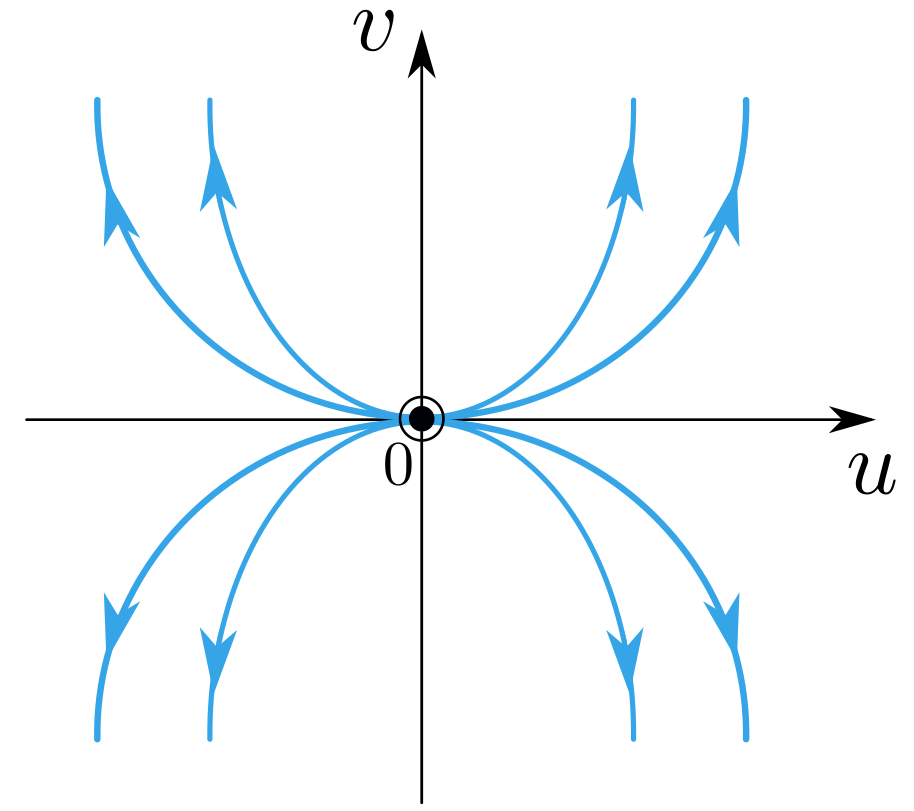
\includegraphics[scale=0.3]{assets/lectures_recent-b13d607a.png} \end{center}

Якщо $ \lambda_2 \cdot \lambda_1 > 0$ та  $ \left| \lambda_2 \right| > \left| \lambda_1 \right|  $ (стрілки до нуля за умови $
 \lambda_1, \lambda_2 < 0$):

 \begin{center} 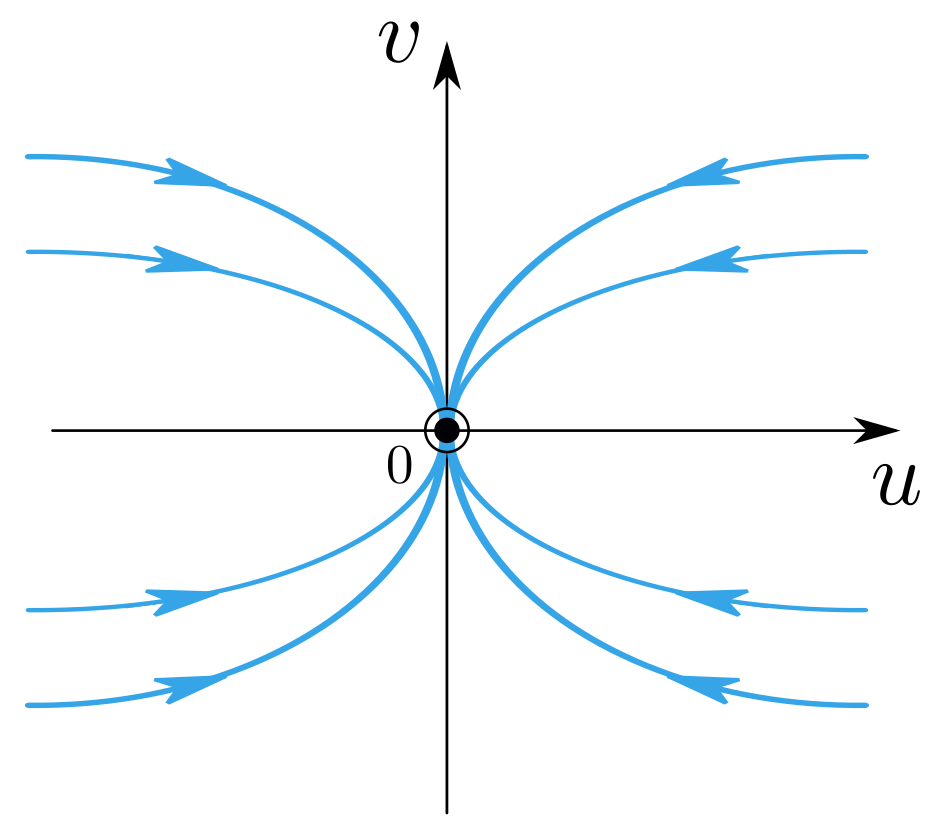
\includegraphics[scale=0.3]{assets/lectures_recent-392ff5ad.png} \end{center}

 Відмітимо, що якщо $\lambda_1, \lambda_2 < 0$, то напрям руху (по $t$) вздовж траєкторій відбувається до нуля. Якщо ж $\lambda_1, \lambda_2 >0$, то рух спрямовано від нуля.\\

 Залишається перейти до початкових змінних $ \begin{bmatrix}
  x \\
   y
 \end{bmatrix}$.\\
Таким чином, якщо $\lambda_1 , \lambda_2 \in \mathbb{R}, \lambda_1 \neq \lambda_2, \lambda_1 \cdot \lambda_2 > 0$ (власні числа одного знаку), то фазовий портрет має вигляд:

\begin{center} 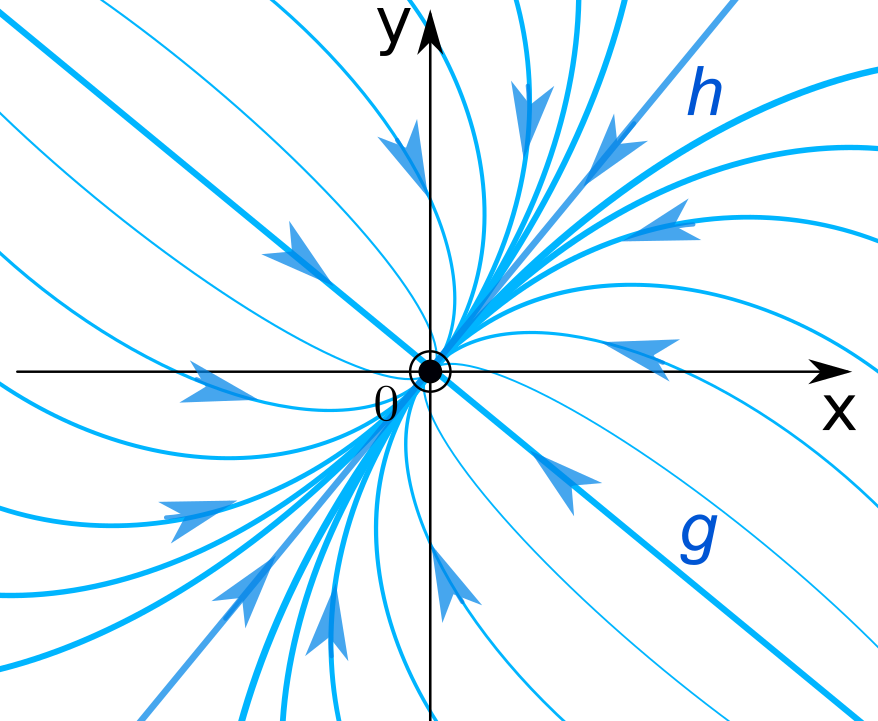
\includegraphics[scale=0.3]{assets/lectures_recent-deaf1762.png} \end{center}

На малюнку $h$ - пряма на якій лежить власний вектор, який відповідає меншому за модулем власному числу.\\
Такий фазовий портрет \textbf{вузол.}\\
- Якщо $\lambda_1, \lambda_2 > 0$ - нестійкий вузол (стрілки від нуля).\\
- Якщо $\lambda_1, \lambda_2 < 0$ - ас. стійкий вузол (стрілки до нуля).

\begin{example}
    $$
    \begin{cases}
    \dot{x} = 2y - 3x\\
    \dot{y} = x - 4y
    \end{cases} \qquad A = \begin{bmatrix}
     -3 & 2 \\
     1 & -4
    \end{bmatrix}
    $$
    $$
    \det{A - \lambda I} = \begin{vmatrix}
      -3 - \lambda & 2 \\
      1 & -4 - \lambda
    \end{vmatrix}  = (-3-\lambda) (-4 - \lambda) -2 = \lambda^2 + 7 \lambda + 10 = 0
    $$
    $$
    \lambda_1 = -2 \qquad \lambda_2 = -5 \Rightarrow \text{ас. стійкий вузол.}
    $$
    Знаходимо власні вектори:\\
    $\lambda_1 = -2$:
    $$
    \begin{bmatrix}
     -1 & 2 \\
     1 & -2
    \end{bmatrix} \begin{bmatrix}
     h_1 \\
     h_2
    \end{bmatrix} = \begin{bmatrix}
     0 \\
     0
    \end{bmatrix} \qquad \begin{gathered}
     -h_1 + 2h_2 = 0\\
     h_1 = 2 h_2
    \end{gathered} \Rightarrow \overline{h} = \begin{bmatrix}
     2 \\
     1
    \end{bmatrix}
    $$
    $\lambda_2 = -5$
    $$
    \begin{bmatrix}
     2 & 2 \\
     1 & 1
    \end{bmatrix} \begin{bmatrix}
     g_1 \\
     g_2
    \end{bmatrix} = \begin{bmatrix}
     0 \\
     0
    \end{bmatrix}
    \qquad \begin{gathered}
     g_1 + g_2 = 0\\
     g_1 = - g_2
    \end{gathered} \Rightarrow \overline{g} = \begin{bmatrix}
     1 \\
     -1
    \end{bmatrix}
    $$

    \begin{center} 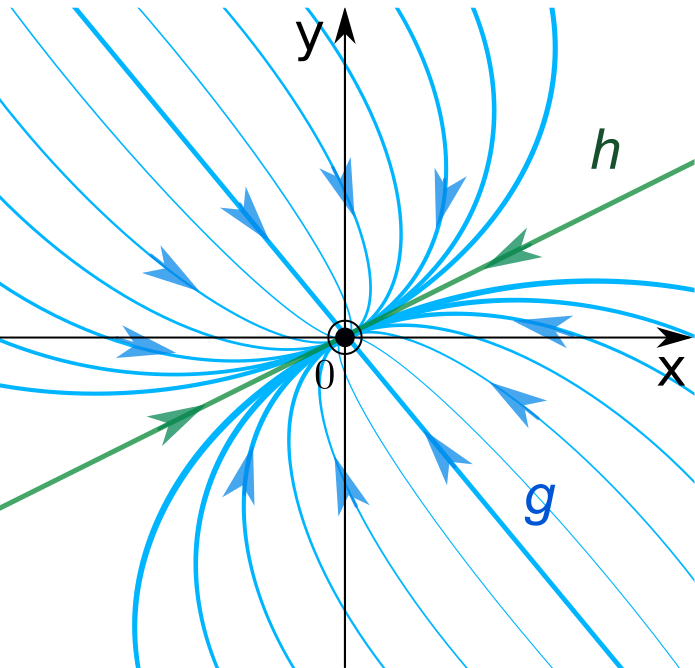
\includegraphics[scale=0.4]{assets/lectures_recent-06adae22.png} \end{center}
\end{example}

2. Нехай $ \lambda_1 , \lambda_2 \in \mathbb{R}, \lambda_1 \neq \lambda_2, \lambda_1 \cdot \lambda_2 < 0$ (Власні числа різних знаків).
Тоді, аналогічно, перейшовши до Жорданового базису, маємо:

$$
\begin{gathered}
\begin{cases}
    \dot{u} = \lambda_1 u\\
    \dot{v} = \lambda_2 v
\end{cases} \\ \begin{cases}
    u = c_1 \cdot e^{\lambda_1 t}\\
    v = c_2 \cdot e^{\lambda_2 t}
\end{cases} \\
 \left[ \begin{array}{l}
v = C \cdot u^{ \frac{\lambda_2}{\lambda_1} }\\
u =0 , v = 0
\end{array} \right.
\end{gathered}\quad
\begin{gathered} 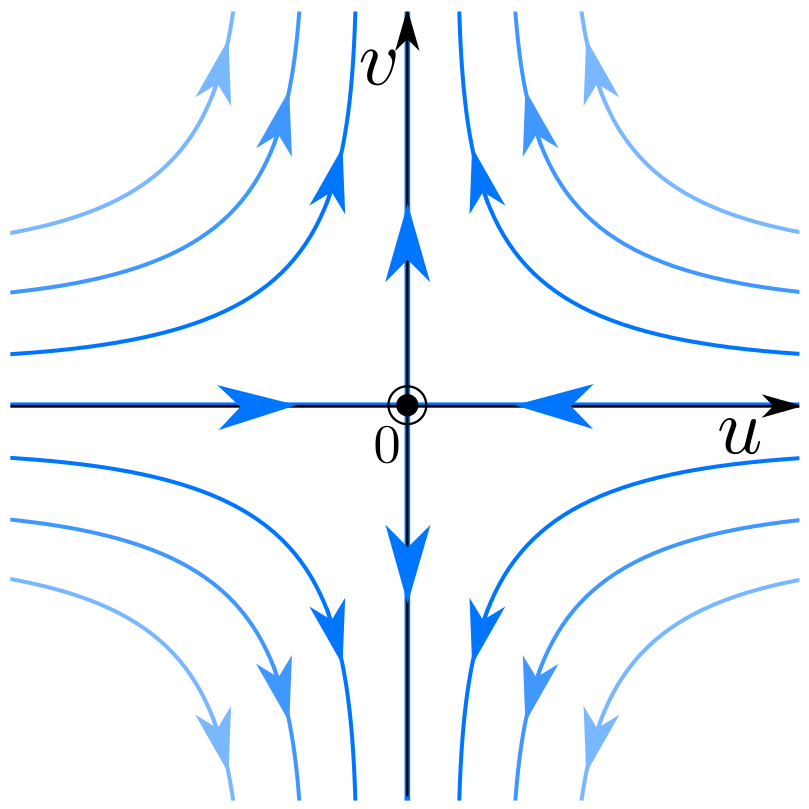
\includegraphics[scale=0.3]{assets/lectures_recent-53a0acd8.png} \end{gathered}
$$


Якщо $ \lambda_1 < 0,
  \lambda_2 > 0
$, то $
 \begin{gathered}
 u(t) \xrightarrow[t \to \infty]{} 0\\
 v(t) \xrightarrow[t \to \infty]{} \infty
 \end{gathered}.$\\
 Якщо $ \lambda_1 < 0,
  \lambda_2 > 0$, то  $
   \begin{gathered}
   u(t) \xrightarrow[t \to \infty]{} \infty\\
   v(t) \xrightarrow[t \to \infty]{} 0
   \end{gathered}.$\\
У другому випадку напрям руху траекторій відбуватиметься в інший бік.\\
Отже, перейшовши до початкових змінних, отримаємо, що за умови $\lambda_1 \cdot \lambda_2 < 0$ фазовий портрет має вигляд:

\begin{center} 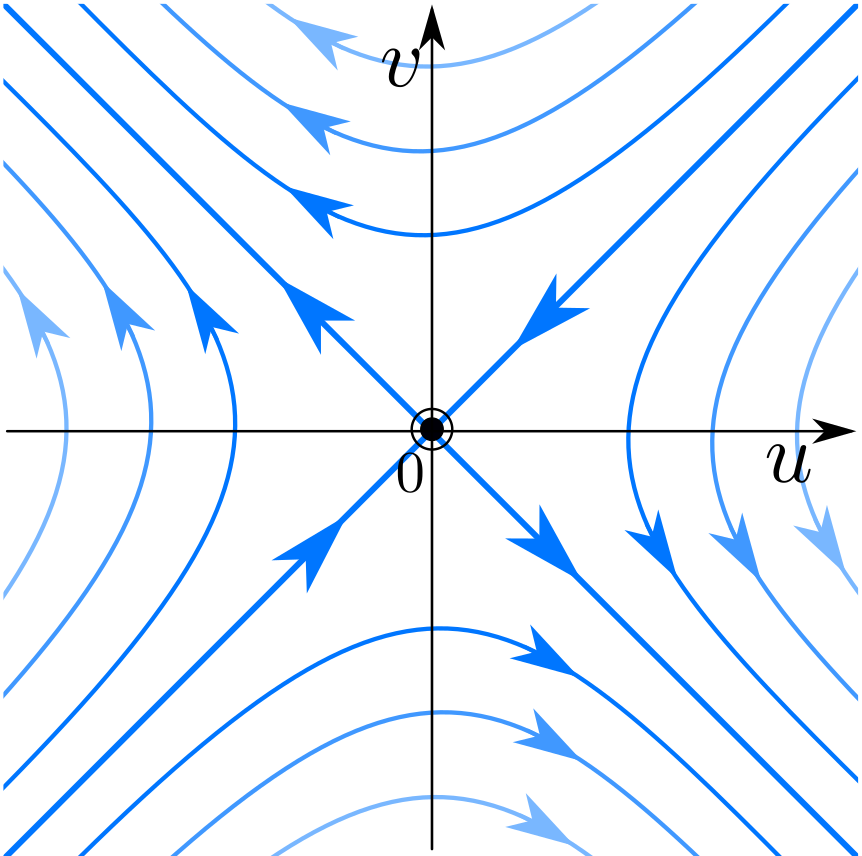
\includegraphics[scale=0.25]{assets/lectures_recent-0ebe704d.png} \end{center}

\begin{remark}
    Стрілки до нуля вздовж прямої, на якій лежить власний вектор, що відповідає $ \lambda_1 < 0$.\\
    Стрілки від нуля вздовж прямої, на якій лежить власний вектор, що відповідає $ \lambda_2 > 0$.
\end{remark}
Такий фазовий портрет називається \textbf{сідло}. Це завжди нестійке положення рівноваги.

\begin{example}
    $$
    \begin{cases}
        \dot{x} = x + 3y\\
        \dot{y} = 2x
    \end{cases} \qquad A = \begin{bmatrix}
     1 & 3 \\
     2 & 0
    \end{bmatrix}
    $$
    $$
    \det (A - \lambda I) = \begin{vmatrix}
      1-\lambda & 3 \\
      2 & - \lambda
    \end{vmatrix} = (1- \lambda)(-\lambda) - 6 = \lambda^2 - \lambda - 6 = 0
    $$
    $$
    \lambda_1 = 3 \quad \lambda_2 = -2 \Longrightarrow \text{сідло (нестійке)}
    $$
    Знаходимо власні вектори:
    $\lambda_1 = 3$
    $$
    \begin{bmatrix}
     -2 & 3\\
     2 & -3
    \end{bmatrix} \begin{bmatrix}
     h_1\\
     h_2
    \end{bmatrix} = \begin{bmatrix}
      0\\
      0
    \end{bmatrix} \qquad 2h_1 = 3 h_2 \Rightarrow \overline{h} = \begin{bmatrix}
     3 \\
     2
    \end{bmatrix}
    $$

    $\lambda_2 = -2$

    $$
    \begin{bmatrix}
     3 &3 \\
     2 & 2
    \end{bmatrix} \begin{bmatrix}
     g_1 \\
     g_2
    \end{bmatrix} = \begin{bmatrix}
     0 \\
     0
    \end{bmatrix} \qquad 2 g_1 =-2 g_2 \Rightarrow \overline{g} = \begin{bmatrix}
     1 \\
     -1
    \end{bmatrix}
    $$
    Отримали такий фазовий портрет:
    \begin{center} 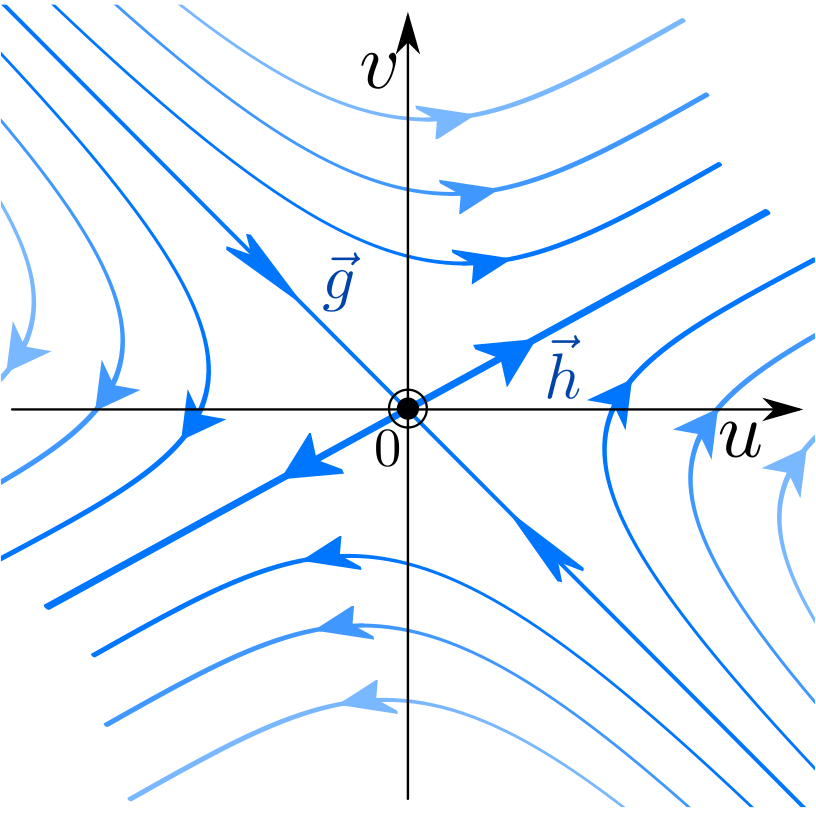
\includegraphics[scale=0.3]{assets/lectures_recent-c4b9c37b.png} \end{center}
    \end{example}


    3. Нехай $ \lambda_1 = \lambda_2 = \lambda \in \mathbb{R}$.\\
    a) Матриця $A$ - діагональна.
    $$
    A = \begin{bmatrix}
     \lambda & 0 \\
     0 & \lambda
    \end{bmatrix} \Longrightarrow \begin{cases}
        \dot{x} = \lambda x\\
        \dot{y} = \lambda y
    \end{cases}
    $$
    В такому випадку, фазовий портрет називають \textbf{диктричний вузол.}




\begin{center} 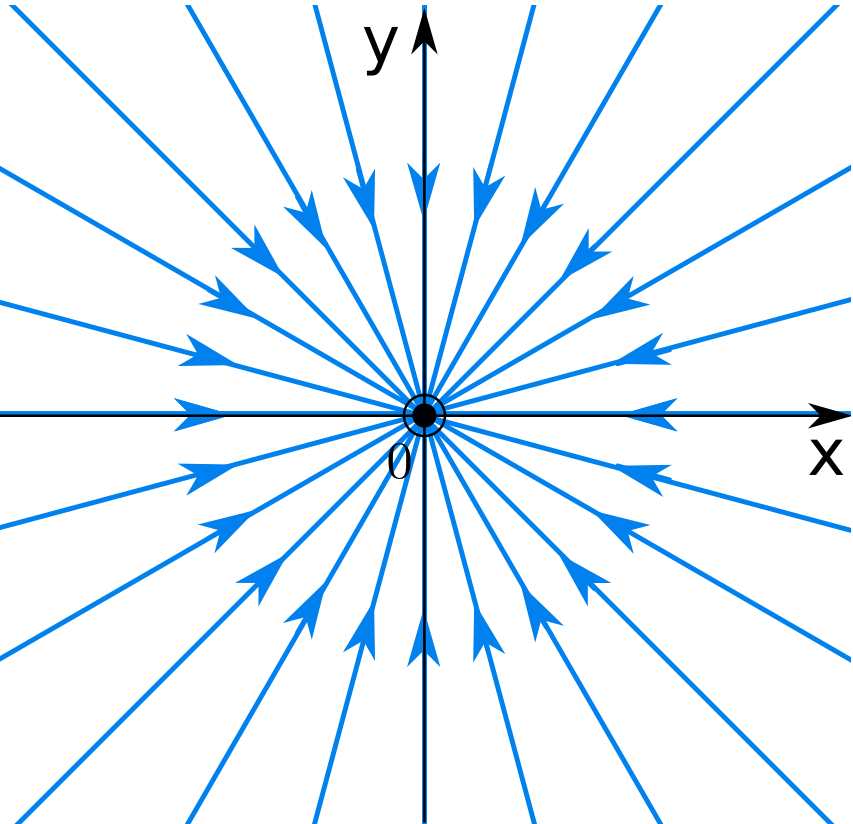
\includegraphics[scale=0.3]{assets/lectures_recent-ab36e3f3.png} \end{center}


Якщо $ \lambda < 0 $ - ас. стійкий (стрілки до нуля).\\
Якщо $ \lambda > 0 $ - нейстійкий (стрілки від нуля). \\
б) Матриця $A$ - недіагональна. В такому разі, фазовий портрет називають \textbf{вироджений вузол.}\\
- якщо $ \lambda < 0 $ - ас. стійкий ( стрілки до нуля ).\\
- якщо $ \lambda > 0 $ - нестійкий (стрілки від нуля).\\
Вироджений вузол може бути двох видів:
\begin{center} 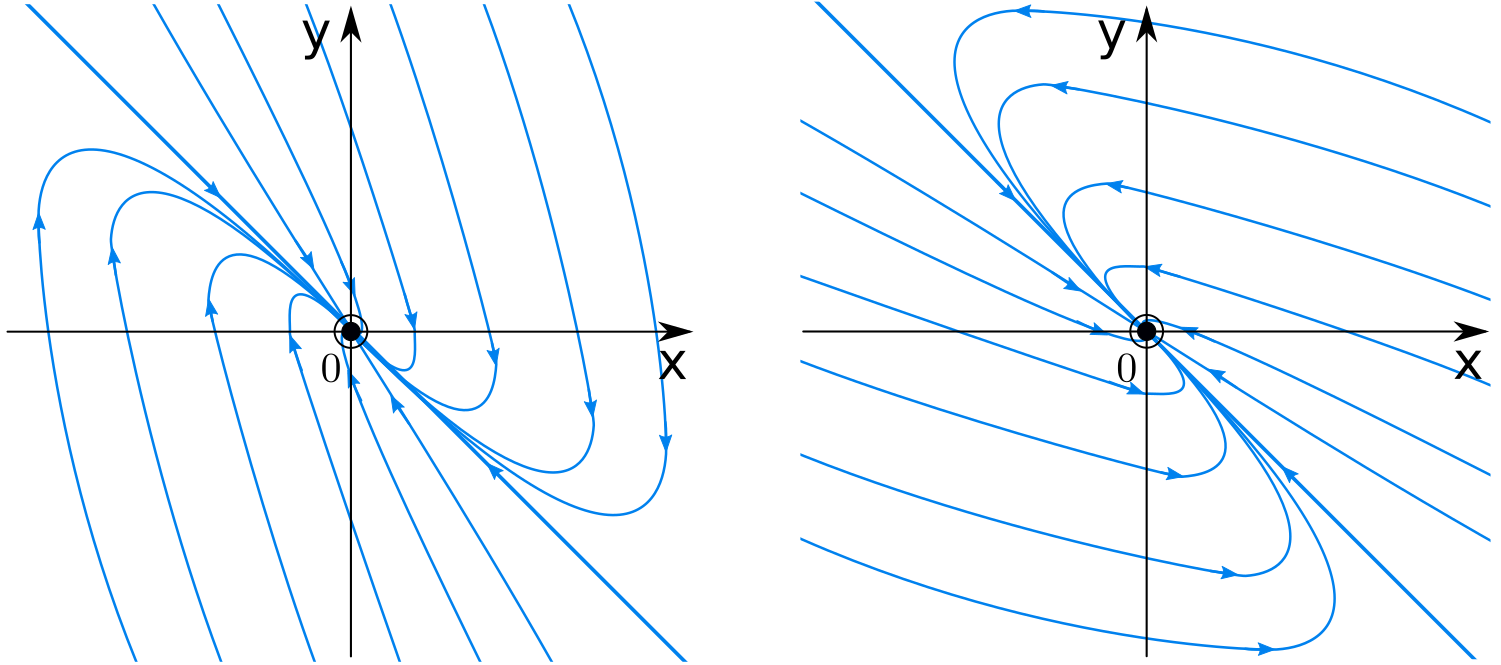
\includegraphics[scale=0.25]{assets/lectures_recent-b526bf37.png} \end{center}

Для визначення типу виродженого вузла потрібно визнгачити напрям вектора фазової швидкості $ \begin{bmatrix}
 \vec{x} \\
 \vec{y}
\end{bmatrix}$ в довільній точці, що не дорівнює нулю системи координат. Цей напрям має співпадати із напрямами руху по фазовій траєкторії (до нуля або від нуля).

\begin{example}
    $$
    \begin{cases}
        \vec{x} = 2y - 3x\\
        \vec{y} = y - 2x
    \end{cases} \qquad A = \begin{bmatrix}
     -3 & 2 \\
     -2 & 1
    \end{bmatrix}
    $$

    $$
    \det{ \left( A - \lambda I  \right) } = \begin{vmatrix}
      -3 - \lambda & 2 \\
      -2 & 1 - \lambda
    \end{vmatrix} = ( -3 - \lambda ) ( 1 -\lambda) + 4 =  \lambda^2 + 2 \lambda + 1 =
    $$
    $$
    = ( \lambda+ 1) ^2 = 0 \Longrightarrow  \lambda = -1 - \text{кратності 2. }
    $$
З попереднього випливає, що фазовим портретом буде асимптотично стійкий вироджений вузол (стрілки до нуля).
Знайдемо власний вектор:
$$
\begin{bmatrix}
 -2 & 2 \\
 2 & 2
\end{bmatrix} \begin{bmatrix}
 h_1 \\
 h_2
\end{bmatrix} = \begin{bmatrix}
 0 \\
 0
\end{bmatrix} \qquad h_1 = h_2 \Rightarrow \overline{h} = \begin{bmatrix}
 1 \\
 1
\end{bmatrix}
$$

\begin{center} 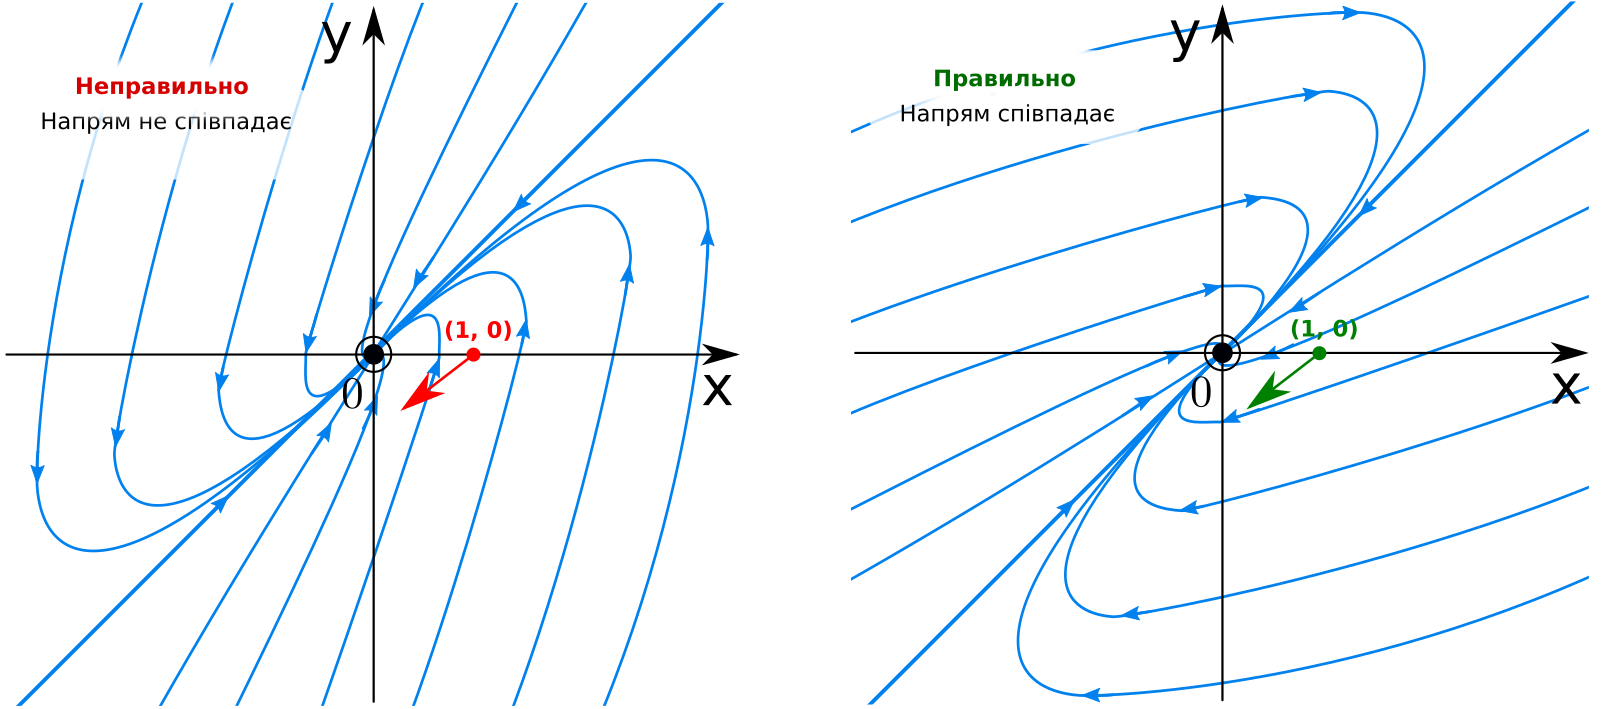
\includegraphics[scale=0.3]{assets/lectures_recent-f0de3cfc.png} \end{center}

Візьмемо т. (1, 0):
$$
\begin{bmatrix}
 \dot{x} \\
 \dot{y}
\end{bmatrix} \Bigg|_{(1,0)} = \begin{bmatrix}
 -3 \\
 -2
\end{bmatrix} \Longrightarrow \begin{gathered}
 x_k = -2 \\
 y_k = -2
\end{gathered}
$$

\end{example}

4. $\lambda_{1, 2} - \alpha \pm i\beta, \alpha\neq 0$. В такому випадку, фазовий портрет назвається \textbf{фокус}. Якщо $ \alpha > 0$ - нестійкий. Якщо $ \alpha > 0$ - ас. стійкий.
Фазовий портрет ''фокус'' може бути двох видів:
\begin{center} 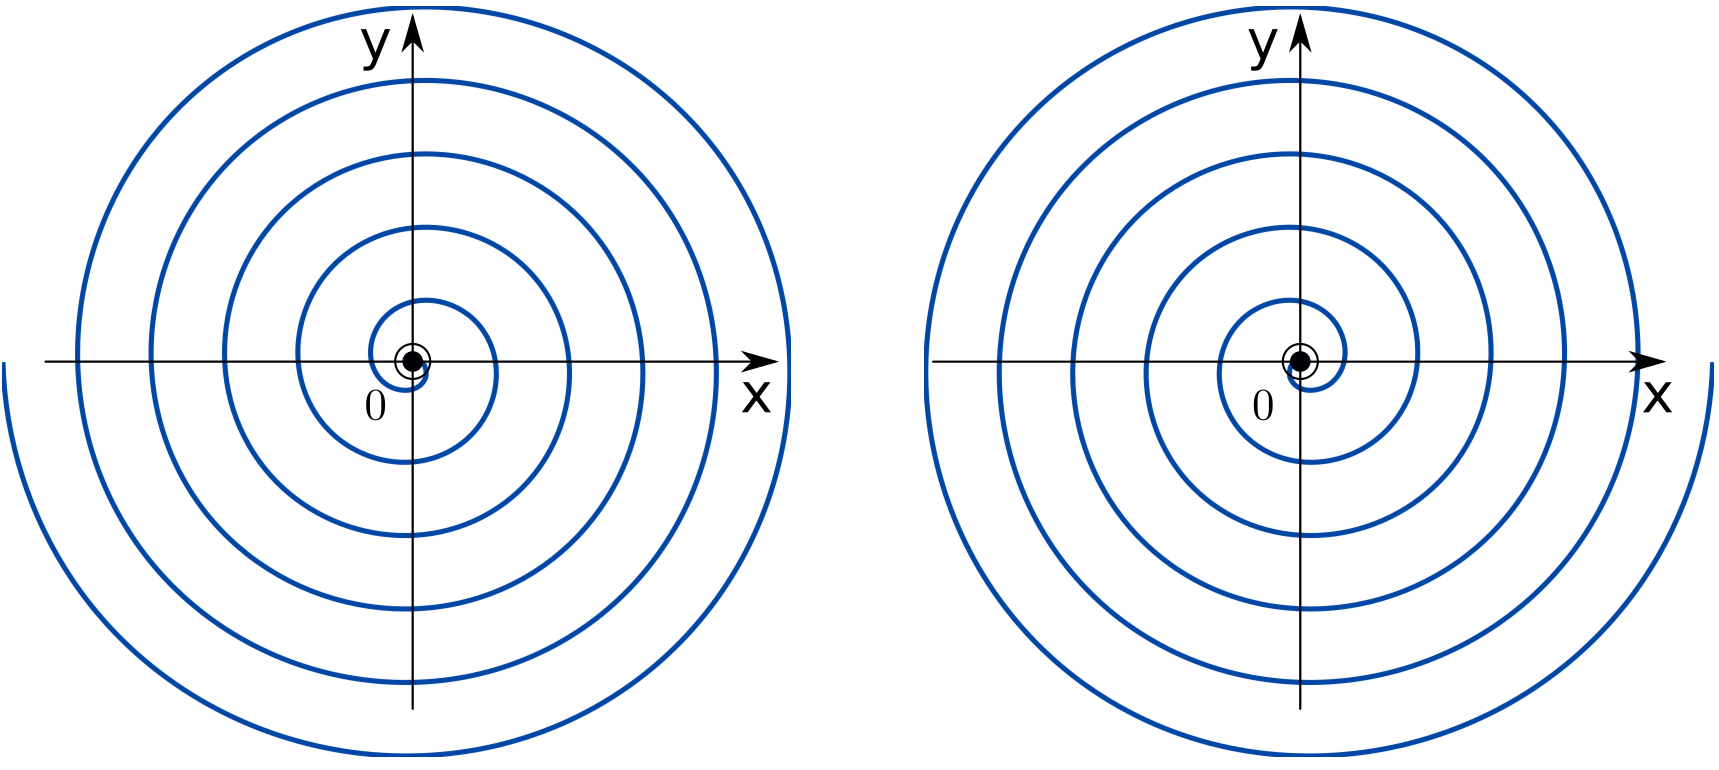
\includegraphics[scale=0.3]{assets/lectures_recent-9fe11a21.png} \end{center}
Для визначення типу фокуса визначаємо напрям вектора фазової швидкості в довільній точці, що не дорівнює нулю.

\begin{example}
    $$
    \begin{cases}
        \dot{x } = x - 2y\\
        \dot{y} = 4x - 3y
    \end{cases} \qquad A = \begin{bmatrix}
     1 & -2 \\
     4 & -3
    \end{bmatrix}
    $$
    $$ \det{(A - \lambda I)} = \begin{vmatrix}
      1- \lambda & -2 \\
      4 & -3-\lambda
    \end{vmatrix}  = ( 1- \lambda) (-3 - \lambda) + 8 = \lambda^2 + 2 \lambda + 5 = 0$$
$$
D = -16 \quad \lambda_{1,2} = \frac{-2 \pm 4i}{2} = -1 \pm 2i
$$
Асимптотично стійкий фокус (стрілки до нуля).
\begin{center} 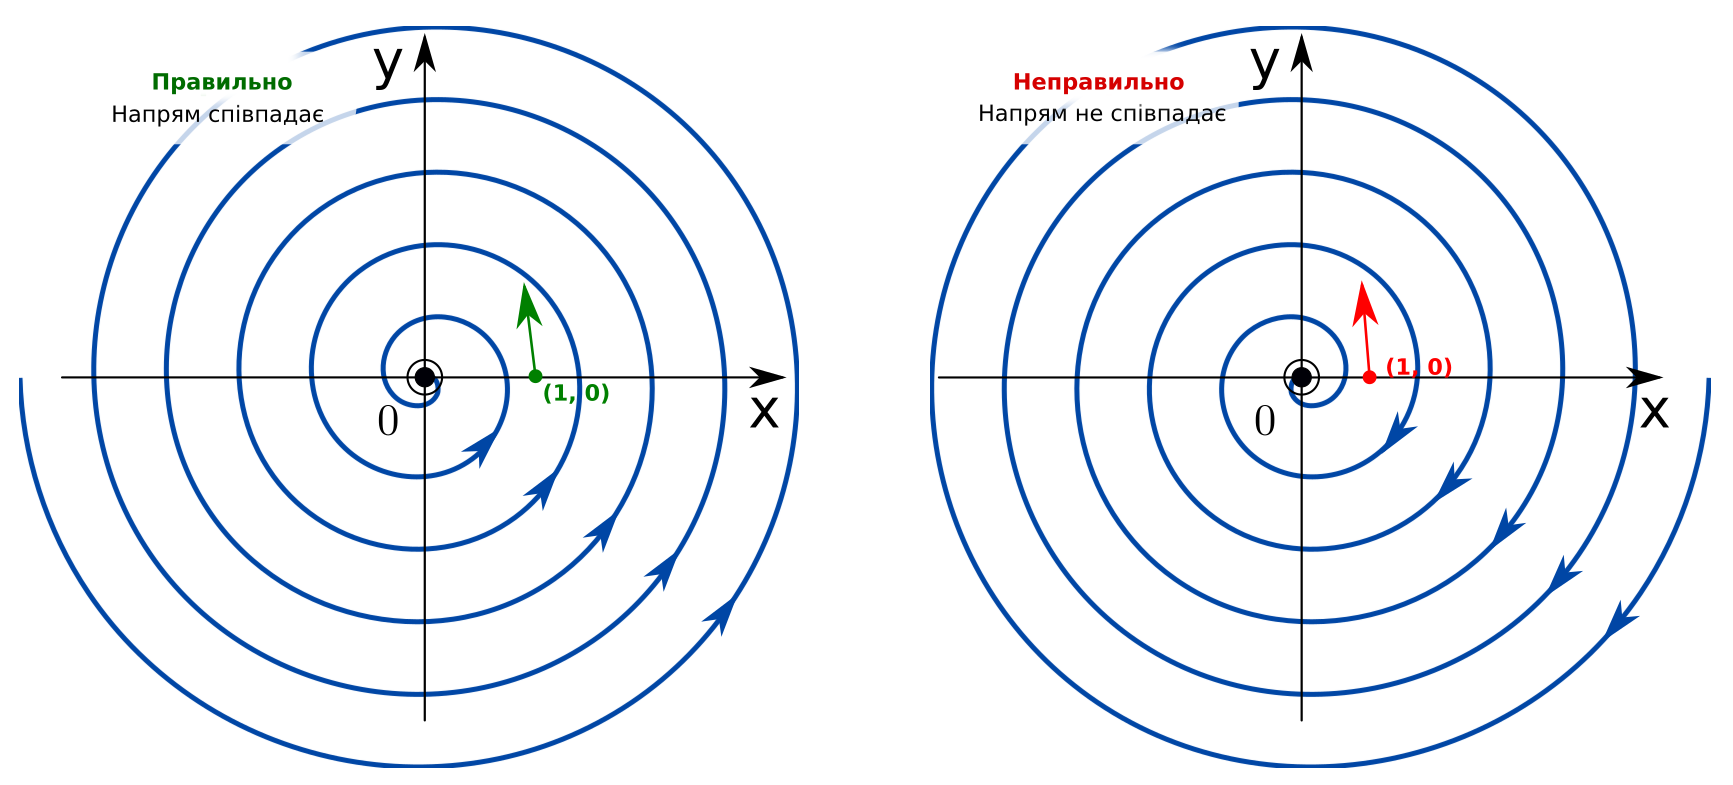
\includegraphics[scale=0.27]{assets/lectures_recent-b90426e3.png} \end{center}
Візьмемо точку (1, 0) для перевірки:

$$
\begin{bmatrix}
 \dot{x}\\
 \dot{y}
\end{bmatrix}\Bigg|_{(1,0)} - \begin{bmatrix}
 1 \\
 4
\end{bmatrix} \qquad \begin{gathered}
 x_k -1 = 1 \\
 y_k - 0 = 4
\end{gathered} \Rightarrow \begin{gathered}
 x_k = 2 \\
 y_k  = 4
\end{gathered}
$$
Отримали: $(1,0) \to (2, 4)$. Перевіримо за виглядом фазового портрета вище.
\end{example}

5.$ \lambda_{1,2} = \pm i \beta$. За таких власних чисел, фазовий портрет називається \textbf{центр.} (стійкий, але не асимптотично стійкий)
\begin{center} 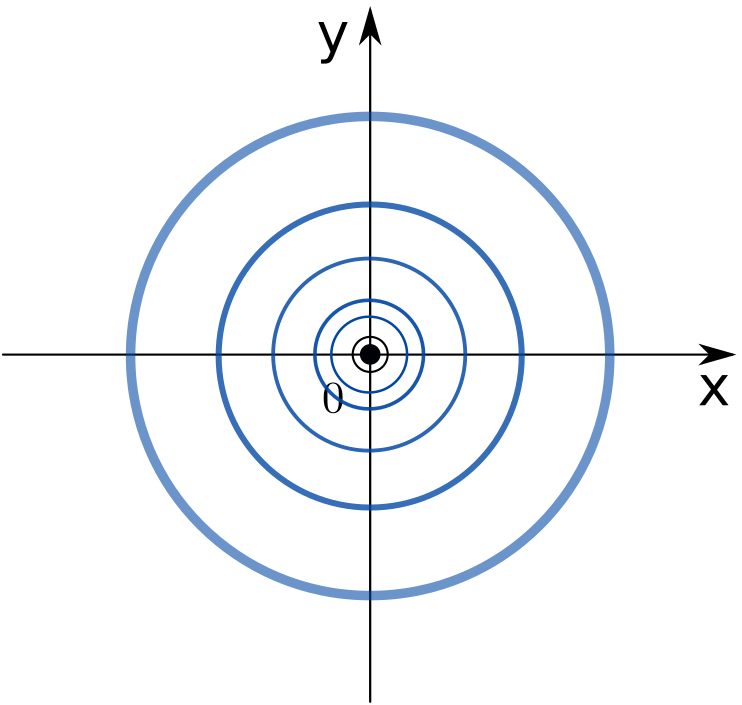
\includegraphics[scale=0.3]{assets/lectures_recent-2982f611.png} \end{center}

\begin{example}
    $$
    \begin{cases}
        \dot{x} = -2 x - 5y \\
        \dot{y} = 2x + 2y
    \end{cases} \qquad A = \begin{bmatrix}
     -2 & -5\\
     2 & 2
    \end{bmatrix}
    $$
    $$
    \det{(A - \lambda I)} = \begin{vmatrix}
      -2-\lambda & -5 \\
      2 & 2 -\lambda
    \end{vmatrix}  = \lambda^2 + 6 = 0 \Rightarrow \lambda = \pm i \sqrt{6} \Rightarrow \text{центр}
    $$
    Візьмемо т. (1, 0):
    $$
\begin{gathered}
\begin{bmatrix}
 \dot{x}\\
 \dot{y}
\end{bmatrix}\Bigg|_{(1,0)} = \begin{bmatrix}
 -2 \\
 2
\end{bmatrix} \\ \begin{cases}
  x_k -1 = -2\\
  y_k  - 0 = 2
\end{cases} \\
\begin{cases}
x_k = -1\\
    y_k  =2
\end{cases}
\end{gathered}\qquad    \begin{gathered} 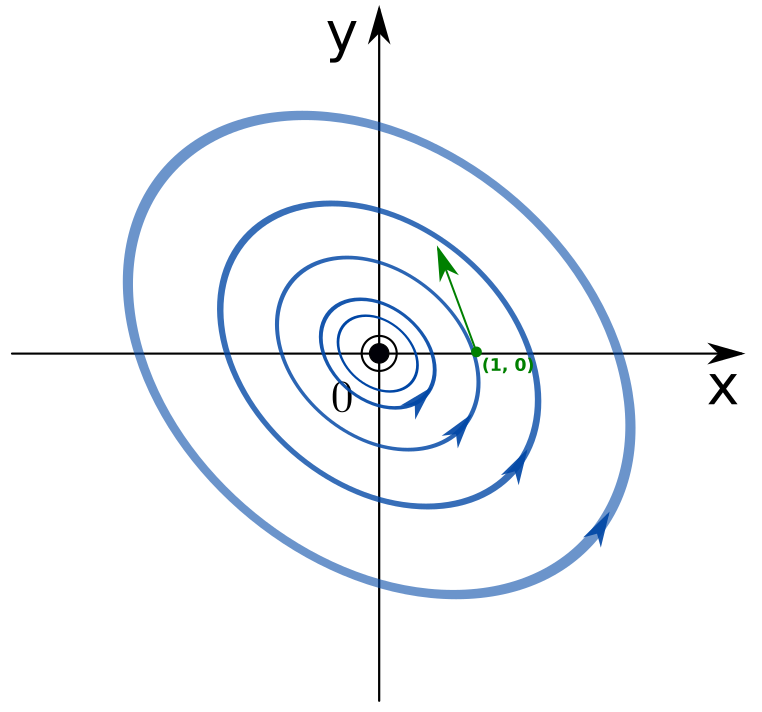
\includegraphics[scale=0.3]{assets/lectures_recent-1467e19e.png} \end{gathered}
    $$


\end{example}
6. Нехай $ \det A = 0$ (вирджений випадок).\\
$$
\det A  =  \begin{vmatrix}
  a & b\\
  c & d
\end{vmatrix} = ad - bc  = 0 \Rightarrow \frac{a}{c} = \frac{b}{d} = 0 \quad \begin{gathered}
 a = kc\\
 b = kd
\end{gathered}
$$
$$
\begin{cases}
    \dot{x} = ax+ by\\
    \dot{y} = k(ax + by)
\end{cases} \Rightarrow ax + by  = 0 \text{ - пряма положень рівноваги.}
$$

$$
\det ( A - \lambda I) = \begin{vmatrix}
  a - \lambda & b\\
  ka & kb - \lambda
\end{vmatrix} = (a-\lambda)*(kb- \lambda) - kab =
$$
$$
 = akb - a \lambda - kb \lambda +  \lambda^2 - kab = \lambda^2 - (a + kb) \lambda =0
 $$
 $$
 \lambda = 0 \qquad \lambda = a + bk
 $$

 a) Прямі паралельні власному вектору, що відповідає власному числу $\lambda =  a + bk$\\
 $\lambda > 0 $ - стрілки від нуля.\\
 $\lambda < 0 $ - стрілки до нуля.\\

 \begin{center} 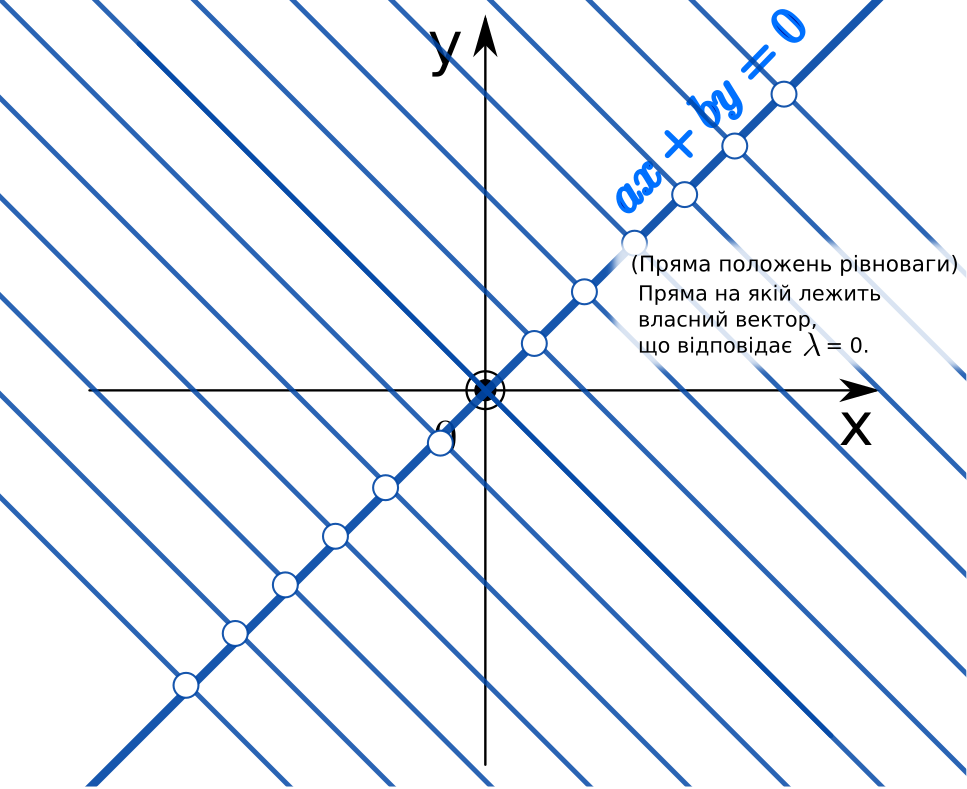
\includegraphics[scale=0.3]{assets/lectures_recent-058ceaff.png} \end{center}
b) $ \lambda_1 =  \lambda_2 = 0 \quad (a = - bk)$

\begin{center} 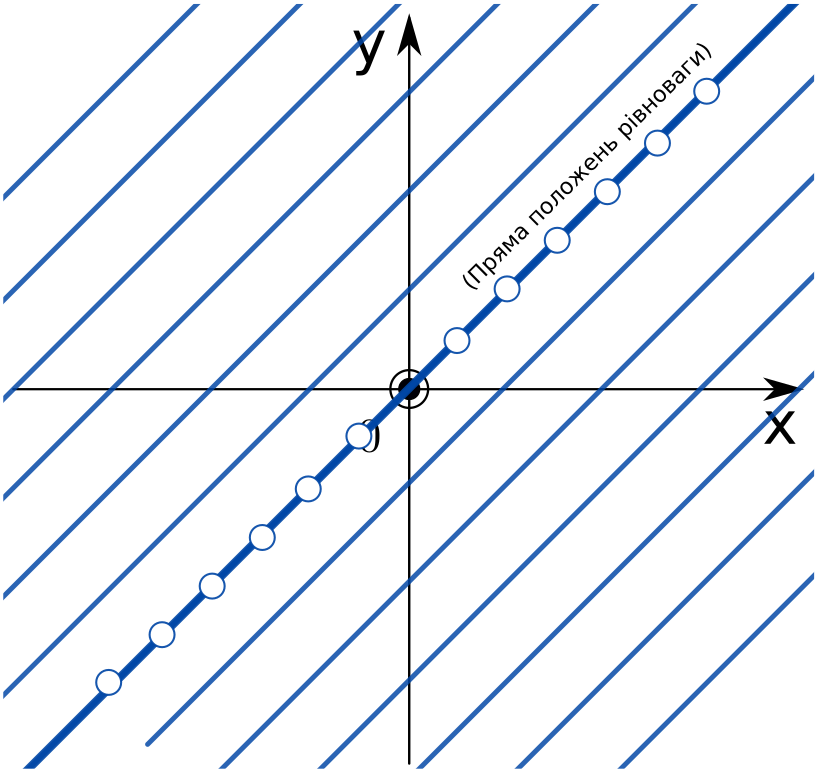
\includegraphics[scale=0.3]{assets/lectures_recent-49093f01.png} \end{center}



\end{document}
